\section{Background}\label{sec:background}

In this section,  we provide the necessary background on reinforcement learning, in both single- and multi-agent settings. 

\subsection{Single-Agent RL}
A reinforcement learning agent is  modeled to perform sequential decision-making by 
interacting with the environment. The environment is usually formulated as an infinite-horizon discounted Markov decision process (MDP), henceforth referred to as Markov decision process\footnote{Note that there are several other standard formulations of MDPs, e.g., time-average-reward setting and finite-horizon episodic setting. Here, we only present the classical infinite-horizon discounted setting for ease of exposition.}, which is formally defined as follows. 
 

\begin{definition}
	A \emph{Markov decision process} is defined by a tuple $(\cS,\cA,\cP,R,\gamma)$, where $\cS$ and $\cA$ denote the state and action spaces, respectively;  $\cP:\cS\times\cA\to\Delta(\cS)$ denotes the transition probability from any state $s\in\cS$ to any state $s'\in\cS$ for any given action $a\in\cA$; $R:\cS\times\cA\times\cS\to\RR$ is the reward function that determines the immediate reward received by the agent for a transition from $(s,a)$ to $s'$; $\gamma\in[0,1)$ is the discount factor that trades off the instantaneous and future rewards. 
\end{definition}


As a standard model, MDP has been widely adopted to characterize the decision-making of an agent with \emph{full observability} of the system state $s$.\footnote{The partially observed MDP (POMDP) model is usually advocated when the agent has no access to the exact system state but only an \emph{observation} of the state. See {\cite{monahan1982state,cassandra1998exact}} for more details on the POMDP model.}  
At each time $t$, the agent chooses to execute an action $a_t$ in face of the system state $s_t$, which causes the system to transition to $s_{t+1}\sim \cP(\cdot\given s_t,a_t)$. Moreover, the agent receives an instantaneous  reward $R(s_t,a_t,s_{t+1})$. 
The goal of solving the MDP is thus to find a policy $\pi:\cS\to\Delta(\cA)$, a mapping from the state space $\cS$ to the distribution over the action space $\cA$, so that $a_t\sim \pi(\cdot\given s_t)$ and the discounted accumulated reward 
\$
\EE\bigg[\sum_{t\geq 0}\gamma^t R(s_t,a_t,s_{t+1})\bigggiven a_t\sim\pi(\cdot\given s_t),s_0\bigg]
\$ is maximized. 
Accordingly, one can define the \emph{action-value function} (Q-function) and \emph{state-value function} (V-function)   under policy $\pi$ as
\$
Q_\pi(s,a) & =\EE\bigg[\sum_{t\geq 0}\gamma^t R(s_t,a_t,s_{t+1})\bigggiven a_t\sim\pi(\cdot\given s_t),a_0=a,s_0=s\bigg], \\
 V_\pi(s) & =\EE\bigg[\sum_{t\geq 0}\gamma^t R(s_t,a_t,s_{t+1})\bigggiven a_t\sim\pi(\cdot\given s_t),s_0=s\bigg]
\$
for any $s\in\cS$ and $a\in\cA$, which are the discounted accumulated reward starting from $(s_0,a_0)=(s,a)$ and $s_0=s$, respectively. The ones corresponding to the optimal policy $\pi^*$ are usually referred to as the \emph{optimal Q-function} and the \emph{optimal state-value  function}, respectively. 

By virtue of the Markovian property, the  optimal policy can be obtained by dynamic-programming/backward induction approaches, e.g., value iteration and policy iteration algorithms \cite{bertsekas2005dynamic}, which require  the knowledge of the model,  i.e., the transition probability and the form of reward function. 
Reinforcement learning, on the other hand,  is to find such an optimal policy without knowing the model. The RL agent learns the policy from experiences collected by interacting with  the environment.  
By and large, RL algorithms can be categorized into two mainstream types, \emph{value-based} and \emph{policy-based} methods. 


\subsubsection{Value-Based Methods} \label{eq:value-based-methods}
Value-based RL methods are devised to find a good estimate of the state-action value function, namely, the optimal Q-function $Q_{\pi^*}$. The (approximate) optimal policy can then be extracted by taking the greedy action of the Q-function estimate. One of the most popular value-based algorithms is Q-learning \cite{watkins1992q}, where the agent maintains an estimate of the Q-value function $\hat{Q}(s,a)$. When transitioning  from state-action pair $(s,a)$  to next state $s'$, the agent receives a payoff $r$ and updates the Q-function according to: 
\#\label{equ:Q_learning}
\hat{Q}(s,a)\leftarrow (1-\alpha)\hat{Q}(s,a)+\alpha\big[r+\gamma\max_{a'}\hat{Q}(s',a')\big],
\#
where  $\alpha>0$ is the stepsize/learning rate. Under certain conditions on $\alpha$, Q-learning can be proved to converge to the optimal Q-value function almost surely \cite{watkins1992q,szepesvari1999unified}, with  finite state and action spaces. Moreover, when combined with neural networks for function approximation, deep Q-learning has achieved great empirical breakthroughs in  human-level control  applications \cite{mnih2015human}. Another popular \emph{on-policy}  value-based method is SARSA, whose convergence  was established in {\cite{singh2000convergence}} for finite-space settings.  

An alternative while popular value-based RL algorithm is Monte-Carlo tree search (MCTS) \cite{chang2005adaptive,kocsis2006bandit,coulom2006efficient}, which estimates the optimal value function by constructing a search tree via Monte-Carlo simulations. Tree polices that 
judiciously select actions to balance exploration-exploitation are used to build and update the search tree. The most common tree policy is to apply the UCB1
(UCB stands for \emph{upper confidence bound})  algorithm, which was  originally devised for stochastic
multi-arm bandit problems \cite{agrawal1995sample,auer2002finite}, to each node of the tree. This yields the popular UCT algorithm \cite{kocsis2006bandit}.  Recent research endeavors on the non-asymptotic convergence of MCTS include \cite{pmlr-v80-jiang18a,shah2019reinforcement}. 
%Convergence guarantee of MCTS  had not been fully characterized until very recently \cite{pmlr-v80-jiang18a,shah2019reinforcement}.   





Besides, another significant task regarding value functions in RL is  to \emph{estimate the value function associated with a  given policy} (not only the optimal one). This task, usually referred to as \emph{policy evaluation}, has been tackled by  algorithms that follow a  similar update as \eqref{equ:Q_learning}, named  \emph{temporal difference} (TD) learning \cite{tesauro1995temporal,tsitsiklis1997analysis,sutton2018reinforcement}. Some other common policy evaluation algorithms with convergence guarantees include gradient TD methods  with linear \cite{sutton2008convergent,sutton2009fast,liu2015finite}, and nonlinear function approximations   \cite{bhatnagar2009convergent}. See \cite{dann2014policy} for a more detailed review on policy evaluation. 

\subsubsection{Policy-Based Methods} \label{sec:policyRL}
Another type of   RL algorithms directly searches over the policy space, which is usually estimated by parameterized function approximators like neural networks, namely, approximating  $\pi(\cdot\given s)\approx\pi_\theta(\cdot\given s)$.  As a consequence, the most  straightforward idea, which is to update the parameter along the gradient direction of the long-term reward, has been instantiated by the  policy gradient (PG) method.    
As a key premise for the idea, the closed-form of PG is given as \cite{sutton2000policy}  
\#\label{equ:policy_grad}
\nabla J(\theta)=\EE_{a\sim\pi_\theta(\cdot\given s),s\sim\eta_{\pi_\theta}(\cdot)}\big[Q_{\pi_\theta}(s,a)\nabla\log\pi_\theta(a\given s)\big],
\#
where $J(\theta)$ and $Q_{\pi_\theta}$ are  the expected return and Q-function under policy $\pi_\theta$, respectively,   $\nabla\log\pi_\theta(a\given s)$ is the score function of the policy, and $\eta_{\pi_\theta}$ is the state occupancy measure, either discounted or ergodic, under policy $\pi_\theta$.  
Then, various policy gradient methods, including  REINFORCE {\cite{williams1992simple}}, G(PO)MDP {\cite{baxter2001infinite}}, and actor-critic algorithms \cite{konda2000actor,bhatnagar2009natural}, have been proposed by estimating the gradient in different ways.  A similar idea also applies to deterministic policies in continuous-action settings, whose PG form has been derived recently  by \cite{silver2014deterministic}. 
Besides gradient-based ones, several other policy optimization methods have achieved state-of-the-art performance in many applications, including PPO  \cite{schulman2017proximal},  TRPO \cite{schulman2015trust}, soft actor-critic \cite{haarnoja2018soft}.  
 

Compared with value-based RL methods, policy-based ones enjoy better convergence guarantees \cite{konda2000actor,yang2018finite,zhang2019global,agarwal2019optimality}, especially with neural networks for function approximation \cite{liu2019neural,wang2019neural}, which can readily handle massive or even continuous state-action spaces.  
Besides the value- and policy-based methods, there also exist RL algorithms based on the linear program formulation of an MDP; see recent efforts in \cite{chen2016stochastic,wang2017primal}. 
   
  
\subsection{Multi-Agent RL Framework}\label{subsec:MARL_framework}

In a similar vein, multi-agent RL  also addresses  sequential decision-making problems, but with more than one agent involved. In particular, both the evolution of the system state and the reward received by each agent are influenced by the joint actions of all agents. More intriguingly, each agent has its own long-term reward to optimize, which now becomes a function of the  policies of all other agents. Such a general model finds broad applications in practice, see \S\ref{sec:applications} for a detailed review of several prominent examples.


In general, there exist two seemingly different but closely related theoretical frameworks for  MARL, Markov/stochastic games and extensive-form games, as to be introduced next. Evolution of the systems under different frameworks are illustrated in Figure \ref{fig:model}. 
 

  
  
  
%\issue{we may need two figures to illustrate these. A system  evolution figure for MGs, and a tree for extensive-form.}

\begin{figure*}[!t]
	\centering 
	\begin{tabular}{ccc} 
		\hskip-25pt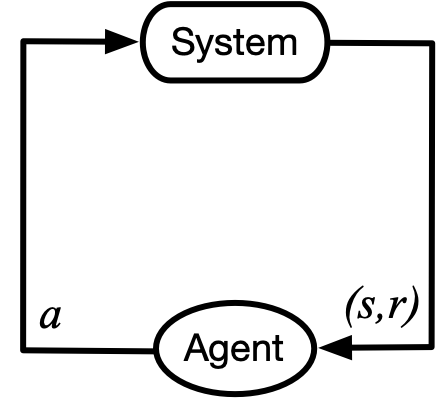
\includegraphics[width=0.28\textwidth]{Fig_1_model_MDP}
		&
		\hskip9pt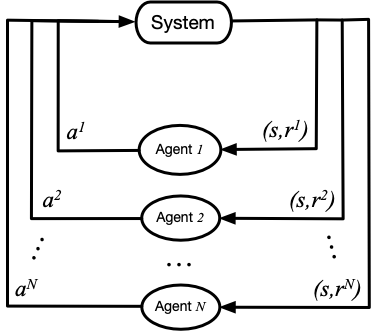
\includegraphics[width=0.31\textwidth]{Fig_1_model_MG}
		& 
		\hskip-17pt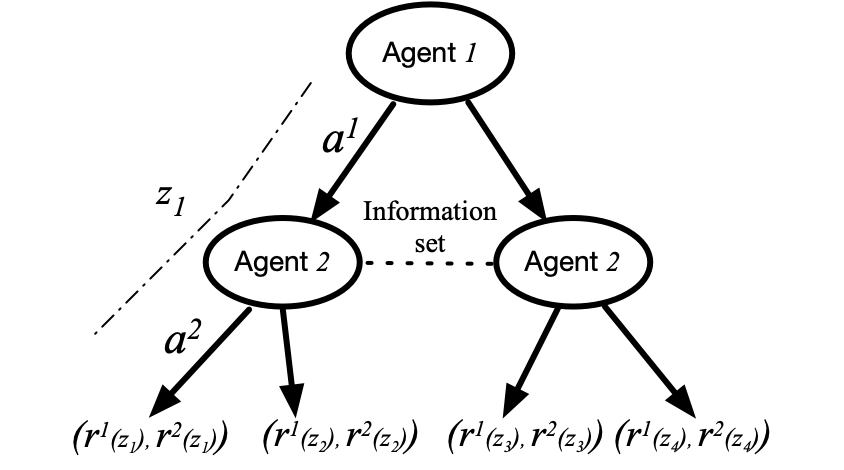
\includegraphics[width=0.44\textwidth]{Fig_1_model_EFG}\\
		\hskip-15pt(a) Markov decision process  & \hskip -2pt(b) Markov game & \hskip-13pt (c) Extensive-form game	\end{tabular}
	\caption{Schematic diagrams for  the system evolution of a Markov decision process, a Markov game, and an extensive-form game, which correspond to the frameworks for single- and multi-agent RL, respectively. Specifically, in an MDP as in (a), the agent observes the state $s$ and receives reward $r$ from the system, after  outputting the action $a$; in an MG as in (b), all agents choose actions $a^i$ simultaneously, after observing the system state $s$ and receiving each individual reward $r^i$; in a two-player extensive-form game as in (c), the agents make decisions on choosing actions $a^i$ alternately, and receive each individual reward $r^i(z)$ at the end of the game, with $z$ being the terminal history. In the  imperfect information case, player $2$ is  uncertain about where he/she is in the game, which makes the information set non-singleton. } 
	\label{fig:model} 
\end{figure*}

 




\subsubsection{Markov/Stochastic Games}\label{subsec:Markov_Games}
%\issue{2019.08.31.}
One direct generalization of MDP that captures the intertwinement of multiple agents is Markov games (MGs),   also known as stochastic games \cite{shapley1953stochastic}. 
Originated from the seminal work \cite{littman1994markov}, the framework of MGs\footnote{Similar to the single-agent setting, here we only introduce the infinite-horizon discounted setting for simplicity, though other settings of MGs, e.g., time-average-reward setting and finite-horizon episodic setting, also exist \cite{filar2012competitive}.} has long been used in the literature  to develop   MARL algorithms, see \S\ref{sec:algorithms} for more details.
We introduce the   formal definition as  below. 


\begin{definition}\label{def:Markov_Game}
	A \emph{Markov game}  is defined by a tuple $(\cN,\cS,\{\cA^i\}_{i\in\cN},\cP,\{R^i\}_{i\in\cN},\gamma)$, where $\cN=\{1,\cdots,N\}$ denotes the set of  $N> 1$ agents, 
	$\cS$ denotes the state space observed by all agents, $\cA^i$ denotes the action space of agent $i$. Let $\cA:=\cA^1\times\cdots\times\cA^N$, then 
	 $\cP:\cS\times\cA\to\Delta(\cS)$ denotes the transition probability from any state $s\in\cS$ to any state $s'\in\cS$ for any joint action $a\in\cA$; $R^i:\cS\times\cA\times\cS\to\RR$ is the reward function that determines the immediate reward received by agent $i$ for a transition from $(s,a)$ to $s'$; $\gamma\in[0,1)$ is the discount factor. 
\end{definition}

At time $t$, each agent $i\in\cN$ executes an action $a^i_t$, according to the system state $s_t$. The system then transitions to state $s_{t+1}$, and rewards each agent $i$ by $R^i(s_t,a_t,s_{t+1})$. The goal of agent $i$ is to optimize its own long-term reward, by finding the policy $\pi^i:\cS\to\Delta(\cA^i)$ such that $a^i_t\sim \pi^i(\cdot\given s_t)$. 
%a mapping from the state space to the probability over its own action space $\cA^i$. 
As a consequence, the value-function $V^i:\cS\to\RR$ of agent $i$   becomes a function of the joint policy $\pi:\cS\to\Delta(\cA)$ defined as $\pi(a\given s):=\prod_{i\in\cN}\pi^i(a^i\given s)$. In particular, for any joint policy $\pi$ and state $s\in\cS$,  
\#\label{eq:V_pi}
V^i_{\pi^i,\pi^{-i}}(s):=\EE\bigg[\sum_{t\geq 0}\gamma^t R^i(s_t,a_t,s_{t+1})\bigggiven a^i_t\sim \pi^i(\cdot\given s_t),s_0=s\bigg],
\#
where $-i$ represents the indices of all agents in $\cN$ except agent $i$. 
%With a random initialization $s_0\sim\cD$ for some distribution  $\cD\in\Delta(\cS)$, the 
Hence, the solution concept of an MG deviates  from that of an MDP, since the \emph{optimal} performance of each agent is controlled not only by its own  policy, but also the choices  of all other  players of the game. The most common solution concept, Nash equilibrium (NE)\footnote{Here, we focus only on stationary Markov Nash equilibria, for the infinite-horizon discounted MGs considered.}, is defined as follows \cite{basar1999dynamic,filar2012competitive}. 

%{\color{red} Maybe use $\eta$ for visitation measure.  consistent with EFG}

\begin{definition}\label{def:NE}
	A \emph{Nash equilibrium} of the Markov game $(\cN,\cS,\{\cA^i\}_{i\in\cN},\cP,\{R^i\}_{i\in\cN},\gamma)$ is a joint policy $\pi^*=(\pi^{1,*},\cdots,\pi^{N,*})$, such that for any $s\in\cS$  and $i\in\cN$
	\$
	V^i_{\pi^{i,*},\pi^{-i,*}}(s)\geq V^i_{\pi^i,\pi^{-i,*}}(s),\quad\text{~~for any~~}\pi^i.
	\$
\end{definition}

Nash equilibrium characterizes an equilibrium  point $\pi^*$, from which none of the agents has any  incentive to deviate. In other words, for any agent $i\in\cN$, the policy $\pi^{i,*} $ is the \emph{best-response} of $\pi^{-i,*}$. As a standard learning goal for MARL, NE always exists for finite-space infinite-horizon discounted MGs \cite{filar2012competitive}, but 
may not be unique in general.  Most of the MARL algorithms are contrived to converge to such an equilibrium point, if it exists. 

%XXX explanaiton of NE XXX 

%Discuss different settings, problem formulation, and solution concept:

The framework of Markov games is general enough to umbrella various MARL settings summarized below. 

\vspace{7pt}
\noindent {\bf Cooperative Setting:}
\vspace{5pt}


In a fully cooperative setting, all agents usually share a common reward function, i.e., $R^1=R^2=\cdots=R^N=R$. 
We note that this model is also  referred to as \emph{multi-agent MDPs} (MMDPs)  in the  AI community \cite{boutilier1996planning,lauer2000algorithm}, and \emph{Markov teams/team Markov games}   in the control/game theory community \cite{yoshikawa1978decomposition,ho1980team,wang2003reinforcement,mahajan2008sequential}. Moreover, from the game-theoretic perspective, this cooperative setting can also be viewed as a special case of Markov \emph{potential} games \cite{gonzalez2013discrete,zazo2016dynamic,valcarcel2018learning}, with the potential function being the common accumulated reward. 
With this model in mind, the value function and Q-function are identical to all agents, which thus enables the single-agent RL algorithms, e.g., Q-learning update \eqref{equ:Q_learning}, to be applied, if all agents are coordinated as one decision maker.  
 The global optimum for cooperation now constitutes a Nash equilibrium of the game.  

Besides the common-reward model, another slightly more general and surging model for cooperative MARL considers  \emph{team-average}  reward \cite{kar2013cal,zhang2018fully,doan2019finitea}. Specifically, agents are allowed to have different reward functions, which may be kept private to each agent, while the goal for cooperation is to optimize  the long-term reward corresponding to the average reward $\bar{R}(s,a,s'):=N^{-1}\cdot \sum_{i\in\cN}R^i(s,a,s')$ for any $(s,a,s')\in\cS\times\cA\times\cS$. The average-reward model, which allows more heterogeneity among agents, includes the model above as a special case.   It also   preserves   privacy among agents, and  facilitates  the development of  \emph{decentralized} MARL algorithms \cite{kar2013cal,zhang2018fully,wai2018multi}. Such heterogeneity also necessitates  the incorporation of \emph{communication} protocols  into MARL, and the analysis of communication-efficient MARL algorithms.


\vspace{7pt}
\noindent {\bf Competitive Setting:}
\vspace{5pt}

Fully competitive setting in MARL is typically modeled as \emph{zero-sum} Markov games, namely, $\sum_{i\in\cN}R^i(s,a,s')=0$ for any $(s,a,s')$. For ease of algorithm analysis and computational tractability, most literature focused on  
\emph{two} agents  that compete  against each other \cite{littman1994markov}, where clearly the reward of one agent is exactly the loss of the other. 
In addition to  direct applications to game-playing \cite{littman1994markov,silver2017mastering,OpenAI_dota_1v1}, zero-sum games also serve as a model for \emph{robust} learning, since the \emph{uncertainty} that impedes the learning process of the agent can be accounted for as 
a fictitious opponent in the game that is always against the agent   \cite{jacobson1973optimal,bacsar1995h,zhang2019policy}. Therefore, the Nash equilibrium yields a robust policy that optimizes the \emph{worst-case} long-term reward. 
%Zero-sum Markov games have been utilized to model a plethora of applications with competitive agents such as video games \cite{}, the game of Go \cite{}, etc. 



\vspace{7pt}
\noindent {\bf Mixed Setting:}
\vspace{5pt}


Mixed setting is also known as the \emph{general-sum} game setting, where no  restriction  is imposed on the goal and relationship among agents \cite{hu2003nash,littman2001friend}. Each agent is self-interested, whose reward may be conflicting  with others'. Equilibrium solution  concepts from game theory, such as Nash equilibrium \cite{basar1999dynamic}, have  the most significant influence on algorithms that are developed for  this general setting.  Furthermore, we include the setting with both fully cooperative and competitive agents, for example, two zero-sum competitive teams with cooperative agents in each team \cite{lagoudakis2003learning,zhang2018finite,OpenAI_dota}, as instances of the mixed setting as well.


%\begin{itemize}
%	\item Cooperative
%	\item Competitive
%	\item Mixed Settings 
%\end{itemize}


\subsubsection{Extensive-Form Games}

Even though they constitute  a classical formalism for MARL, Markov games can only handle the fully observed case, i.e., the agent has \emph{perfect information} on the system state $s_t$ and the executed action $a_t$ at time $t$. Nonetheless, a plethora of  MARL applications involve agents with only partial observability, i.e., \emph{imperfect information} of the game. 
Extension of Markov games to partially  observed case may be applicable, which, however, is challenging to solve, even under the cooperative setting \cite{oliehoek2016concise,bernstein2002complexity}.\footnote{Partially observed Markov games under the cooperative setting are usually formulated as decentralized POMDP (Dec-POMDP) problems. See \S\ref{subsec:partially_observed} for more discussions on this setting.}    
%{\color{red} Why challenging? Because policies need to take the whole histories as the input, which is not scalable?}
  
In contrast, another framework, named  \emph{extensive-form games} \cite{osborne1994course,shoham2008multiagent}, can handily model imperfect information for multi-agent decision-making. This framework is  rooted in   computational game theory  and has been  shown to admit polynomial-time algorithms under mild conditions \cite{koller1992complexity}. We briefly introduce the framework of extensive-form games as follows.    
%{\color{red} What the logic? EFG can be viewed as an extension of static game, which models game with a tree structure such as poker. What makes EFG solvable?}

\begin{definition} \label{def:ext_form_game}
	An \emph{extensive-form game}  is  defined by   $(\cN\cup \{c\},\cH,\cZ,\cA, \{ R^i\}_{i \in \cN},\tau,\pi^c,\cS)$, where $\cN = \{ 1, \ldots, N \}$ denotes the set of $N > 1 $ agents, and $c$ is a special agent called \emph{chance} or \emph{nature},  which has a fixed stochastic policy that specifies the randomness of the environment.  Besides,  $\cA$ is the set of all possible actions that agents can take and $\cH$ is the set of all possible \emph{histories}, where each history is  a sequence of actions taken  from the beginning of the game. 
	Let     $\cA(h)=\{a\given ha \in\cH\}$ denote  the set of  actions available after a nonterminal history $h $. 
	Suppose an agent takes action $a \in \cA(h)$ given  history $h \in \cH$, which then leads to a  new history $ha \in \cH$. 
	Among all histories, $\cZ\subseteq \cH$ is a subset of \emph{terminal histories} that represents the completion of a game. 
%	At each terminal history, 
%	rewards are assigned to each agent in $\cN$. Particularly, for each $i \in \cN $, let 
A utility is assigned to each agent $i \in \cN$ at a terminal history, dictated by the function 
	$R^i \colon  \cZ\rightarrow \RR$. 
%	 is the reward function of agent $i\in\cN$, namely, the reward is assigned  to each agent at the terminal history.  
	 Moreover, $\tau :\cH\to\cN\cup \{c\}$ is the \emph{identification} function that specifies which agent takes the action at each history. 
%	 to specify which agent takes the action at each history, let $\tau :\cH\to\cN\cup \{c\}$ be  the \emph{identification} function
%	such that agent $\tau(h)$ takes action at history $h$. 
	If $\tau(h)=c$, the chance agent takes an  action $a$  according to its policy $\pi^c$, i.e., $a \sim \pi^c(\cdot\given h)$. Furthermore, $\cS$ is the partition of $\cH$ such that  
%	 the imperfect information of an agent about the game is represented by a  partition $\cS$ of $\cH$ based on the agents' observations. 
%	 Specifically, 
	 for any $s \in \cS$ and any $h, h' \in s $,  we have  $\tau(h) = \tau(h') $ and  $\cA (h) = \cA (h')$. In other words, histories $h$ and $h'$ in the same partition are indistinguishable to the agent that is about to take action, namely $\tau(h)$. The elements in $\cS$ are referred to as 
	 \emph{information states}.
	\end{definition}

Intuitively, the imperfect information of  
an extensive-form game is reflected by the fact that  agents cannot distinguish between histories in the same information set. 
%It reduces to a perfect information game if every information set is a singleton. 
Since we have $\tau(h) = \tau(h') $ and  $\cA (h) = \cA (h')$ for all $h,h'\in s$ and $s\in\cS$,  
for ease of presentation,  in the sequel, for all $h \in s$, 
%we let   $\cA(h)=\{a\given ha \in\cH\}$ denote  the set of  actions available after a nonterminal history $h$, and 
we let $\cA(s) $ and $\tau(s)$ denote  $\cA (h)$ and $\tau(h)$, respectively. We also define a mapping $I \colon \cH \rightarrow \cS$ by letting $I (h) = s$ if $h \in s$. 
Moreover, we only consider games   where both  $\cH$  and $\cA$ are   finite sets. To simplify the notation, for any two histories $h, h' \in \cH$, we refer to $h$ as a \emph{prefix} of $h'$, denoted by $h  \sqsubseteq h'$,   if $h'$ can be reached from $h$ by taking a sequence of actions. In this case, we call $h'$ a \emph{suffix} of $h$. 
Furthermore, we assume throughout that 
the game features  \emph{perfect recall}, which  implies that  each agent remembers the sequence of the information states and  actions that have led to  its current information state.
The assumption of perfect recall is commonly made in the literature, which enables the existence of polynomial-time algorithms for solving the game \cite{koller1992complexity}. 
More importantly, by the celebrated 
Kuhn's theorem \cite{kuhn1953extensive}, under such an assumption, to find the set of  
Nash equilibria, it suffices to    restrict  the derivation  to the set of \emph{behavioral policies} which map each information set $s \in \cS$ to a probability distribution over $\cA (s)$. For any $i \in \cN$, let $\cS^i = \{ s\in \cS \colon \tau(s) = i \}$ be the set of information states of agent $i$. A joint policy of the agents is denoted by  $\pi = ( \pi^1, \ldots, \pi^N )  $, where  $\pi^i:\cS^i\to \Delta ( \cA (s) )$ is the policy of agent $i$. 
%is a mapping defined on $\cS^i$ such that  $\pi^i (\cdot \given s)  \in \Delta ( \cA (s) )$ for any $s \in \cS^i$. 
For any history $h$ and any joint policy $\pi$, we define the 
 \emph{reach probability} of $h$ under $\pi$  as 
\#\label{eq:reach_prod}
\eta _\pi (h) = \prod  _{h' \colon h'a\sqsubseteq h } \pi^{\tau(h')}    (a\given I(h')   ) =  \prod_{i \in \cN \cup \{c\}} \prod_{h' \colon h'a \sqsubseteq h, \tau(h') = i } \pi^i   (a \given I(h')  ),
\# 
 which specifies the probability that $h$ is created when all agents follow $\pi$. 
 We similarly define the reach probability of an information state $s $ under $\pi$ as $\eta_\pi (s) = \sum_{h \in s} \eta_\pi (h)$. The expected utility of agent $i \in \cN$ is  thus given by  $     \sum_{ z \in \cZ } \eta_\pi(z) \cdot R^i (z) $, which is denoted by $R^i ( \pi)  $ for simplicity. 
 Now we are ready to introduce  the solution concept for  extensive-form games, i.e., 
Nash equilibrium and its $\epsilon$-approximation, as follows. 
%  for an extensive-form game.    


\begin{definition}\label{def:extens_NE}
	An \emph{$\epsilon$-Nash equilibrium} of an extensive-form game represented by $(\cN\cup \{c\},\cH,\cZ,\\\cA, \{ R^i\}_{i \in \cN},\tau,\pi^c,\cS)$  is a joint policy $\pi^*=(\pi^{1,*},\cdots,\pi^{N,*})$, such that for any 
	%	$s\in\cS$  and 
	$i\in\cN$, 
	\$
	R^i (\pi^{i,*}, \pi^{-i,*})  \geq R^i ( \pi^i, \pi^{-i,*}) 
	 -\epsilon,\quad\text{~~for any policy~}\pi^i \text{~of agent }i.
	\$
	 Here   $\pi ^{-i}$ denotes the joint policy of    agents in  $\cN \setminus \{ i\} $ where agent $j$ adopts policy $\pi^j$ for all $j \in  \cN \setminus \{ i\}$.  Additionally, if $\epsilon=0$, $\pi^*$ constitutes a \emph{Nash equilibrium}. 
\end{definition}


\begin{comment}
\vspace{25pt}
{\color{red} XXXX  Revise accordingly.  }
\begin{definition}\label{def:ext_form_game}
	An \emph{extensive-form game} is defined by   $(\cN\cup \{c\},\cH,\cZ,\cA,u,\tau,f_c,\cS)$, where 
	\begin{itemize}
	  \setlength\itemsep{-0.2em}
		\item $\cN=\{1,\cdots,N\}$ denotes the set of $N> 1$ agents, and $c$ denotes a special agent \emph{chance};
		\item $\cH$ denotes a finite set of \emph{histories}, with each history being a sequence of actions taken from the beginning of the game; $\cZ\subseteq \cH$ is a subset of \emph{terminal histories} that represents the completion of a game;
		\item $\cA$ denotes the set of all   actions that agents can take, and $\cA(h)=\{a\given (h,a)\in\cH\}$ denotes the actions available after a nonterminal history $h$;
		\item $u:\cZ\to \Delta_u^N\subseteq\RR^N$ denotes the function that assigns utility to each agent for a given terminal state, where $\Delta_u\in[u_{\min},u_{\max}]$ is the interval of utility lying between the minimum $u_{\min}$ and maximum $u_{\max}$;
		\item $\tau:\cH\to\cN\cup \{c\}$ denotes the \emph{agent identity} function, so that if $\tau(h)\in\cN$, it  identifies which agent acts after the history $h\in\cH$; if $\tau(h)=c$, the chance agent determines the action taken after history $h$, according to the probability given by $f_c(\cdot\given h)$; 
		\item $\cS=\{\cS^1,\cdots,\cS^N\}$ denotes the set of \emph{information partitions} $\cS^i$, where $\cS^i$ is a  partition of $\{h\in\cH\given \tau(h)=i\}$ such that $\cA(h)=\cA(h')$ whenever $h$ and $h'$ are in the same member of the partition. For any $s^i\in\cS^i$, let $\cA(s^i)=\cA(h)$ and $\tau(s^i)=\tau(h)$ for any $h\in s^i$. The set $s^i\in\cS^i$ is referred to as the \emph{information set/state} of agent $i$.
	\end{itemize}
%	$\cS$ denotes the set of (information)  states, which  is a partition of $\cH$ such that each $s\in\cS$ contains histories $h\in s$ that cannot be distinguished by $\tau(h)$ for all $h\in s$. Thus, one can define $\tau(s)=\tau(h)$ for any $h\in s$.
\end{definition}


%By definition,  $\cS$ can be partitioned according to the agents in $\cN$ into $\cS^1,\cdots,\cS^N$. 
The decision of each  agent $i$ is then made upon the information state $s^i\in\cS^i$. Particularly, $s^i$ determines the action set $\cA(s^i)$ available to the agent, and 
%, since some actions may be private and not revealed to other agents at state $s$; 
$\pi^i:\cS^i\to \Delta(\cA(s^i))$, the   policy of agent $i$, maps  from the information state space $\cS^i$.  
%The chance agent 
Nash equilibrium and its $\epsilon$-approximation can also be used as 
the solution concept here, as defined below. 


\begin{definition}\label{def:extens_NE}
	An \emph{$\epsilon$-Nash equilibrium} of an extensive-form game $(\{\cN,c\},\cH,\cA,\cZ,u,\tau,\cS)$  is a joint policy $\pi_*=(\pi^1_*,\cdots,\pi^N_*)$, such that for any 
%	$s\in\cS$  and 
	$i\in\cN$
	\$
	\EE_{\pi^i_*,\pi^{-i}_*}\big(u^i\big)\geq \EE_{\pi^i,\pi^{-i}_*}\big(u^i\big)-\epsilon,\quad\text{~~for any~~}\pi^i,
	\$
	for any $\epsilon\geq 0$. If $\epsilon=0$, $\pi_*$ constitutes a \emph{Nash equilibrium}. 
\end{definition}
\end{comment}

\vspace{7pt}
\noindent {\bf Various Settings:}
\vspace{5pt}

Extensive-form games are in general used to model non-cooperative settings. 
%can also model all cooperative, competitive, and mixed settings, by assuming various structures on the utility function $R$. Explicitly, identical utility function with $R^1=R^2=\cdots=R^N$ leads to the fully cooperative setting; 
Specifically, zero-sum/constant-sum utility with $\sum_{i\in\cN}R^i=k$ for some constant $k$ corresponds to the fully competitive setting; general-sum utility function results in the mixed setting.  
More importantly, settings of different information structures can also be characterized  by   extensive-form games. In particular, a \emph{perfect information} game is  one where each information set is a singleton, i.e., for any $s\in\cS$, $|s|=1$;  an \emph{imperfect information} game is  one where  there exists $s\in\cS$, $|s|>1$. In other words, with  imperfect information, the information state $s$ used for decision-making represents more  than one possible history, and the agent cannot distinguish between them. 

Among various settings, the zero-sum imperfect information setting has been the main focus of theoretical studies that bridge MARL and extensive-form games \cite{zinkevich2008regret,heinrich2015fictitious,srinivasan2018actor,omidshafiei2019neural}. It has also motivated MARL algorithms that  revolutionized competitive  setting applications like Poker AI \cite{rubin2011computer,brown2019superhuman}. 


\vspace{7pt}
\noindent {\bf Connection to Markov Games:}
\vspace{5pt}

Note that the two formalisms in Definitions \ref{def:Markov_Game} and \ref{def:ext_form_game} are connected. In particular, for simultaneous-move Markov games, the choices of actions by other agents are unknown to an agent, which thus  leads  to different histories that can be aggregated as one information state $s$. Histories in these games are then  sequences of \emph{joint} actions, and the discounted accumulated reward instantiates the utility at the end of the game. 
Conversely, by simply setting $\cA^j=\emptyset$ at the state $s$ for agents $j\neq \tau(s)$, the extensive-form game reduces to a Markov game with \emph{state-dependent} action spaces. See \cite{lanctot2019openspiel} for a more detailed discussion on the  connection.

%Based on recent efforts that associate MARL with computational game theory, 

\begin{remark}[Other MARL Frameworks]
	{{Several other theoretical frameworks for MARL also exist in the literature, e.g.,  normal-form and/or  repeated games  \cite{claus1998dynamics,bowling2001rational,kapetanakis2002reinforcement,conitzer2007awesome}, and partially observed Markov games \cite{hansen2004dynamic,amato2013decentralized,amato2015scalable}. 
However, the former framework can be viewed as a special case of MGs, with a singleton state; most early theories of  MARL in this framework have been   restricted to small scale problems  \cite{bowling2001rational,conitzer2007awesome,kapetanakis2002reinforcement} only. 
MARL in the latter framework, on the other hand, is inherently challenging to address in general \cite{bernstein2002complexity,hansen2004dynamic}, leading to relatively scarce theories in the literature.   Due to space limitation,   we do not introduce these models here  in any detail. We will briefly review  MARL algorithms under some of these models, especially the partially observed setting, in    \S\ref{sec:algorithms}, though. Interested readers are referred to  the early review \cite{bu2008comprehensive} for more discussions on MARL in normal-form/repeated games. }}
\end{remark}  
